% !TEX root = ../presentation.tex
% !BIB program = biber
% !TEX program = xelatex

\section{a brief overview of unsupervised speech representation learning}

% \setbeamerfont{itemize/enumerate body}{}
% \setbeamerfont{itemize/enumerate subbody}{size=\small}
% \setbeamerfont{itemize/enumerate subsubbody}{size=\footnotesize}

\begin{frame}
    \frametitle{\vphantom{ABCDEFGHJIJKLMNOPQRSTVWXYZ}{Development of SSL for speech}}
    \begin{columns}[t]
        \hspace{0.025\textwidth}
        \begin{column}{0.20\textwidth}
            \begin{figure}[\textwidth]
                \centering
                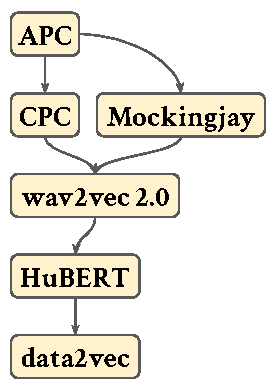
\includegraphics[width=\textwidth]{figures/brief-flow-0.pdf}
            \end{figure}
        \end{column}
        {\textcolor{black!40}{\vrule{}}}
        % \vphantom{%
        %     \begin{column}{0.40\textwidth}
        %         {\vspace{0.10\textheight}\footnotesize#3}
        %     \end{column}
        %     \begin{column}{0.30\textwidth}
        %         \begin{figure}[\textwidth]
        %             \centering
        %             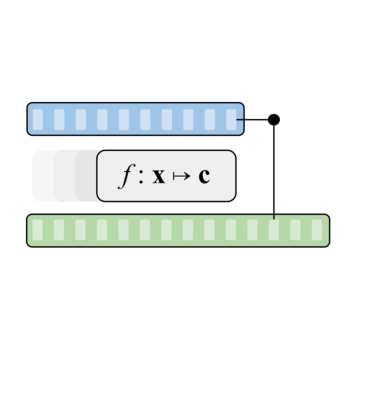
\includegraphics[width=\textwidth]{figures/brief-model-1.pdf}
        %         \end{figure}
        %     \end{column}
        % }{\hphantom{%
        %     \begin{column}{0.40\textwidth}
        %         {\vspace{0.10\textheight}\footnotesize#3}
        %     \end{column}
        %     \begin{column}{0.30\textwidth}
        %         \begin{figure}[\textwidth]
        %             \centering
        %             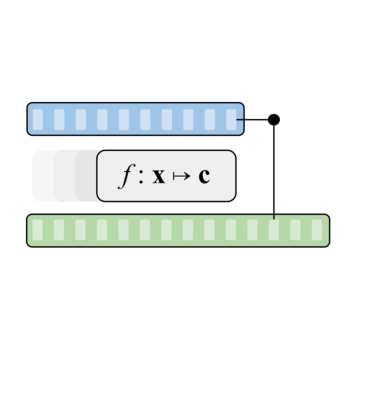
\includegraphics[width=\textwidth]{figures/brief-model-1.pdf}
        %         \end{figure}
        %     \end{column}
        % }{
        \begin{column}{0.70\textwidth}
            \centering
            \begin{figure}[\textwidth]
                \centering
                {\vspace{0.2\textheight}\color{black!40}\scshape model description goes here}
            \end{figure}
        \end{column}
        % }}
        % \begin{column}{0.4\txtwidth}
            % \vspace{0.1\textheight}
            % {\footnotesize #3}
        % \end{column}
        % \hfill
        % \hspace{0.050\textwidth}
        % \begin{column}{0.65\textwidth}
        %     \begin{figure}[\textwidth]
        %         \centering
        %         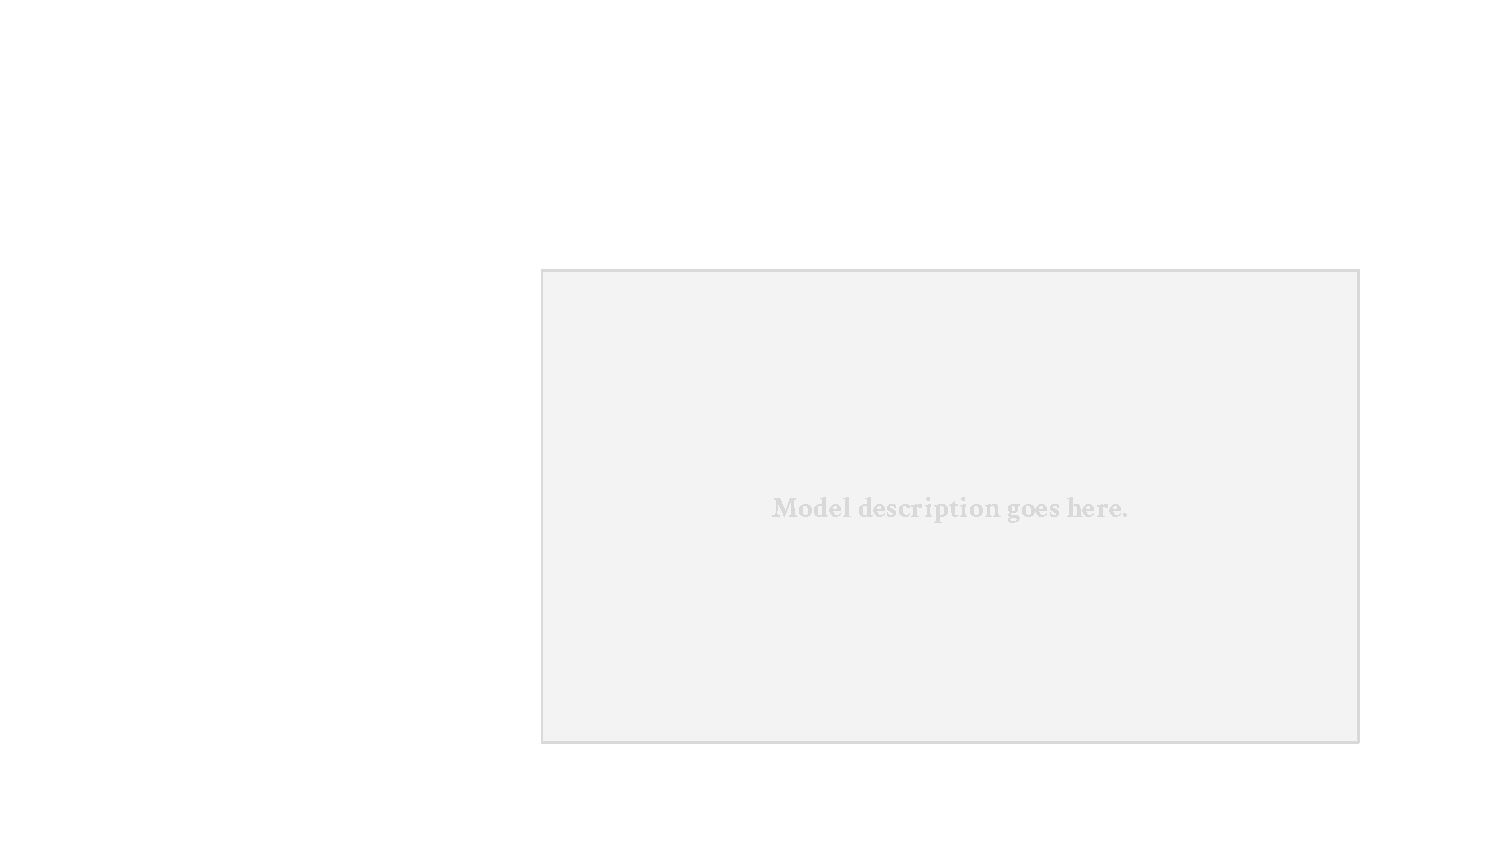
\includegraphics[width=\textwidth]{figures/brief-model-0.pdf}
        %     \end{figure}
        % \end{column}
        % \hfill
        \hspace{0.020\textwidth}
    \end{columns}
\end{frame}

{ % start font size change group

\setbeamerfont*{itemize/enumerate body}{size=\fontsize{8}{10}}
\setbeamerfont*{itemize/enumerate subbody}{parent=itemize/enumerate body}
\setbeamerfont*{itemize/enumerate subsubbody}{parent=itemize/enumerate body}

\newcommand{\presentationbriefslide}[3]{%
    \begin{frame}
        \frametitle{\vphantom{ABCDEFGHJIJKLMNOPQRSTVWXYZ}{#2}}
        \begin{columns}[t]
            \hspace{0.025\textwidth}
            \begin{column}{0.20\textwidth}
                \begin{figure}[\textwidth]
                    \centering
                    \includegraphics[width=\textwidth]{figures/brief-flow-#1.pdf}
                \end{figure}
            \end{column}
            {\textcolor{black!40}{\vrule{}}}
            \begin{column}{0.40\textwidth}
                {\vspace{0.10\textheight}\footnotesize#3}
            \end{column}
            \begin{column}{0.30\textwidth}
                \begin{figure}[\textwidth]
                    \centering
                    \includegraphics[width=\textwidth]{figures/brief-model-#1.pdf}
                \end{figure}
            \end{column}
            \hspace{0.020\textwidth}
        \end{columns}
    \end{frame}
}

% \presentationbriefslide{0}{Development of SSL for speech}{}%

\presentationbriefslide{1}{Autoregressive Predictive Coding (APC)}{%
    \begin{itemize}
        \item {\bfseries \color{black} Task}: Predict future inputs.
        \item {\bfseries \color{black} Input/target}: Log-mel spectrogram.
        \item {\bfseries \color{black} Architecture}: RNN/Transformer decoder.
        \item {\bfseries \color{black} Slow features}: Predict $k$ steps ahead.
    \end{itemize}
}

\presentationbriefslide{2}{Autoregressive Predictive Coding (APC)}{%
    \begin{itemize}
        \item {\bfseries \color{black} Challenges}:
        \begin{itemize}
            \item Encodes only past inputs \xmark
            \item Uses the input as target \xmark
        \end{itemize}
    \end{itemize}
}

\presentationbriefslide{3}{Mockingjay}{%
    \begin{itemize}
        \item {\bfseries \color{black} Task}: Reconstruct masked inputs.
        \item {\bfseries \color{black} Architecture}: Transformer encoder.
        \item {\bfseries \color{black} Masking}: 
        \begin{itemize}
            \item $X$\% at random. (Mockingjay)
            \item $X$\% + $N$ consecutive (wav2vec 2.0)
            \item SpecAugment (Masked RNN)
        \end{itemize}
    \end{itemize}
}

\presentationbriefslide{4}{Mockingjay}{%
    \begin{itemize}
        \item {\bfseries \color{black} Challenges}:
        \begin{itemize}
            \item Encodes the entire input \cmark
            \item Uses the input as target \xmark
        \end{itemize}
    \end{itemize}
}

\presentationbriefslide{5}{Contrastive Predictive Coding (CPC)}{%
    \begin{itemize}
        \item {\bfseries \color{black} Contrastive models}: Distinguish target samples from negative samples.
        \item {\bfseries \color{black} Learned target}: Discard details.
        \item {\bfseries \color{black} Sampling negatives}:
        \begin{itemize}
            \item Sample sequence?
            \item Same speaker?
        \end{itemize}
    \end{itemize}
}

\presentationbriefslide{6}{Contrastive Predictive Coding (CPC)}{%
    \begin{itemize}
        \item {\bfseries \color{black} Challenges}:
        \begin{itemize}
            \item <1-> Only encodes past inputs \xmark
            \item <1-> Uses a learned target \cmark
            \item <2-> Sampling negatives \xmark
        \end{itemize}
    \end{itemize}
}

\presentationbriefslide{8}{wav2vec 2.0} WER.
            \item 10 mimutes: \textbf{4.8\%} WER.
        \end{itemize}
    \end{itemize}
}

\presentationbriefslide{9}{wav2vec 2.0}{%
    \begin{itemize}
        \item {\bfseries \color{black} Challenges}:
        \begin{itemize}
            \item Encodes the entire input \cmark
            \item Uses a learned target \cmark
            \item Sampling negatives \xmarkshaded
        \end{itemize}
    \end{itemize}
}

\presentationbriefslide{10}{Hidden-unit BERT (HuBERT)}{%
    \begin{itemize}
        \item {\bfseries \color{black} Target}: $K$-means teacher.
        \item {\bfseries \color{black} Training}: Simple cross-entropy loss.
        \item {\bfseries \color{black} 1st iteration}: $K$-means on inputs.
    \end{itemize}
}


\presentationbriefslide{11}{Hidden-unit BERT (HuBERT)}{%
    \begin{itemize}
        \item {\bfseries \color{black} Target}: $K$-means teacher.
        \item {\bfseries \color{black} Training}: Simple cross-entropy loss.
        \item {\bfseries \color{black} 1st iteration}: $K$-means on inputs.
        \item {\bfseries \color{black} 2nd iteration}: $K$-means on hidden layers.
    \end{itemize}
}


\presentationbriefslide{12}{Hidden-unit BERT (HuBERT)}{%
    \begin{itemize}
        \item {\bfseries \color{black} Challenges}:
        \begin{itemize}
            \item <1-> Encodes the entire input \cmark
            \item <1-> Uses a learned target \cmark
            \item <1-> No need for negative samples \cmark
            \item <2-> Targets updated infrequently \xmark
            \item <2-> Quantized targets \xmark
        \end{itemize}
    \end{itemize}
}

\presentationbriefslide{14}{data2vec}{%
    \begin{itemize}
        \item Uses a teacher-student framework.
        \item {\bfseries \color{black} Teacher}:
        \begin{itemize}
            \item EMA of student (online) \cmark
            \item Target is average of top $K$ layers \cmark
        \end{itemize}
    \end{itemize}
}

\presentationbriefslide{15}{data2vec}{%
    \begin{itemize}
        \item Uses a teacher-student framework.
        \item {\bfseries \color{black} Teacher}:
        \begin{itemize}
            \item EMA of student (online) \cmark
            \item Target is average of top $K$ layers \cmark
        \end{itemize}
        \item {\bfseries \color{black} Student training}: Smooth $\l_1$ loss.
    \end{itemize}
}

\presentationbriefslide{16}{data2vec}{%
    \begin{itemize}
        \item {\bfseries \color{black} Challenges}:
        \begin{itemize}
            \item Encodes the entire input \cmark
            \item Uses a learned target \cmark
            \item No need for negative samples \cmark
            \item Targets updated continuously \cmark
            \item Continuous-valued targets \cmark
        \end{itemize}
    \end{itemize}
}

} % end font size change group

% \setbeamerfont*{itemize/enumerate body}{}
% \setbeamerfont*{itemize/enumerate subbody}{}
% \setbeamerfont*{itemize/enumerate subsubbody}{}

\begin{frame}
    \frametitle{Conclusions}
    \begin{itemize}
        \item {\bfseries Main conclusions}:
        \begin{itemize}
            \item The most popular self-supervised speech models can be compactly described by a few core design choices.
            \item Many of these design choices are mirrored in earlier work on speech embedding models.
        \end{itemize}
        \item {\bfseries Open questions and limitations}:
        \begin{itemize}
            \item Which design choices benefit which downstream tasks?
            \item It is difficult to compare methods as model size and evaluation procedures differ widely between papers.
        \end{itemize}
    \end{itemize}
\end{frame}
